\textbf{Цель работы:} исследование спектра колебаний электрических сигналов.

\textbf{В работе используются:} персональный  компьютер; USB-осциллограф  АКИП-4107; функциональный генератор WaveStation2012; соединительные кабели.
                    
\section{Теоретическое введение}

Используется разложение в сумму синусов и косинусов с различными аргументами или, как чаще его называют, \textit{разложение в ряд Фурье}.

Пусть задана функция $f(t)$, которая периодически повторяется с частотой $\Omega_1 = \dfrac{2\pi}{T}$, где $T$ --- период повторения импульсов. Её разложение в ряд Фурье имеет вид 

\begin{equation}
    f(t) = \dfrac{a_0}{2} + \sum\limits_{n = 1}^{\infty}\left[a_n \cos \left(n \Omega_1t\right) + b_n \sin \left(n \Omega_1t\right)\right]
\end{equation}

или

\begin{equation}
    f(t) = \dfrac{a_0}{2} + \sum\limits_{n = 1}^{\infty}A_n \cos \left(n\Omega_1t-\psi_n\right).
\end{equation}

Если сигнал чётен относительно $t = 0$, в тригонометрической записи остаются только члены с косинусами. Для нечетной наоборот.

Коэффициенты определяются по формуле

\begin{equation}
    \begin{array}{c}
        a_n  = \dfrac{2}{T}\int\limits_{t_1}^{t_1+T}f(t)\cos\left(n \Omega_1 t\right) dt,\\
        \\
        b_n = \dfrac{2}{T}\int\limits_{t_1}^{t_1+T}f(t)\sin\left(n \Omega_1 t\right) dt.
    \end{array}
\end{equation}

Здесь $t_1$ -- время, с которого мы начинаем отсчет.

Сравнив формулы $(1)$ и $(2)$ можно получить выражения для $A_n$  и $\psi_n$:

\begin{equation}
    \begin{array}{l}
        A_n = \sqrt{a_n^2+b_n^2},\\
        \psi_n = \arctan \dfrac{b_n}{a_n}.
    \end{array}
\end{equation}

\subsection{Периодические прямоугольные импульсы}

\begin{figure}[h!]
    \centering
    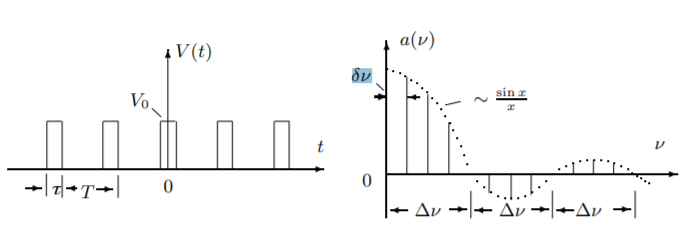
\includegraphics[width = 12 cm]{images/theor_1.png}
    \caption{График сигнала и его спектра (прямугольный импульс)}
    \label{theor_1}
\end{figure}

Введем величину: $\Omega_1 = \dfrac{2\pi}{T}$,
где $T$ -- период повторения импульсов.

Коэффициенты при косинусных составляющих будут равны

\begin{equation}
    a_n = \dfrac{2}{T} \int \limits_{-\tau/2}^{\tau/2} V_0 \cos \left( n \Omega_1 t \right) dt = 2V_0\dfrac{\tau}{T}\dfrac{\sin\left(n\Omega_1\tau/2\right)}{n\Omega_1\tau/2} \sim \dfrac{\sin x}{x}.
\end{equation}

Здесь $V_0$ - амплитуда сигнала.

Поскольку наша функция четная, то $b_n = 0$. 

Пусть $T$ кратно $\tau$. Тогда введем ширину спектра, равную $\Delta \omega$ -- расстояние от главного максимума до первого нуля огибающей, возникающего, как нетрудно убедиться при $n = \dfrac{2\pi}{\tau \Omega_1}$. При этом

\begin{equation}
    \Delta \omega \tau \simeq 2\pi \Rightarrow \Delta \nu \Delta t \simeq 1.
\end{equation}

\subsection{Периодическая последовательность цугов}

\begin{figure}[h!]
    \centering
    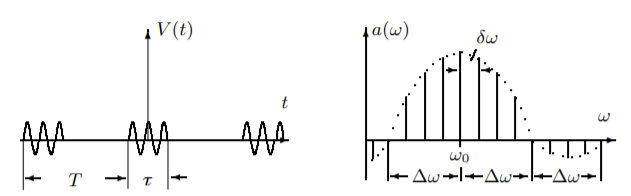
\includegraphics[width = 12 cm]{images/theor_2.png}
    \caption{График сигнала и его спектра (цуг)}
    \label{theor_2}
\end{figure}

Возьмём цуги колебания $V_0 \cos(\omega_0 t)$ с длительностью цуга $\tau$ и периодом повторений $T$.

Функция $f(t)$ снова является четной относительно $t = 0$. Коэффициент при $n$-ой гармонике согласно формуле $(3)$ равен

\begin{equation}
    a_n = \dfrac{2}{T}\int\limits_{-\tau/2}^{\tau/2}V_0 \cos \left(\omega_0t\right) \cdot \cos\left(n \Omega_1t\right)dt = 
\end{equation}

\[ 
    = V_0 \dfrac{\tau}{T}\left( \dfrac{\sin\left[\left(\omega_0 - n \Omega_1\right)\dfrac{\tau}{2}\right]}{\left( \omega_0 - n \Omega_1\right) \dfrac{\tau}{2}} + \dfrac{\sin\left[\left(\omega_0 + n \Omega_1\right)\dfrac{\tau}{2}\right]}{\left( \omega_0 + n \Omega_1\right) \dfrac{\tau}{2}}\right).
\]

Пусть $T$ кратно $\tau$. Тогда спектры последовательности прямоугильных сигналов и цугов аналогичны, но максимумы сдвинуты на $\omega_0$.

\subsection{Амплитудно-модулированные колебания}

\begin{figure}[h!]
    \centering
    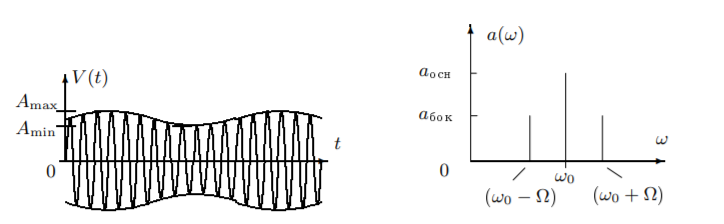
\includegraphics[width = 12 cm]{images/theor_3.png}
    \caption{Пример амплитудной модуляции}
    \label{theor_3}
\end{figure}

Рассмотрим гармонические колебания высокой частоты $\omega_0$, амплитуда которых медленно меняется по гармоническому закону с частотой $\Omega \ll \omega_0$.

\begin{equation}
    f(t) = A_0 \left[1+m\cos \Omega t\right] \cos \omega_0 t.
\end{equation}

Коэффициент $m$ называется \textit{глубиной модуляции}. При $m < 1$ амплитуда меняется от минимальной $A_{min} = A_0(1-m)$ до максимальной $A_{max} = A_0(1+m)$. Глубина модуляции может быть представлена в виде

\begin{equation}
    m = \dfrac{A_{max}-A_{min}}{A_{max}+A_{min}}.
\end{equation}

Простым тригонометрическим преобразованием уравнения $(8)$ можно найти спектр колебаний

\begin{equation}
    f(t) = A_0 \cos \omega_0t + \dfrac{A_0m}{2} \cos \left(\omega_0 + \Omega\right)t + \dfrac{A_0m}{2}\cos\left(\omega_0 - \Omega\right)t.
\end{equation}

\section{Обработка данных}

\subsection{Периодические прямоугольные импульсы}

\begin{figure}[h!]
    \centering
    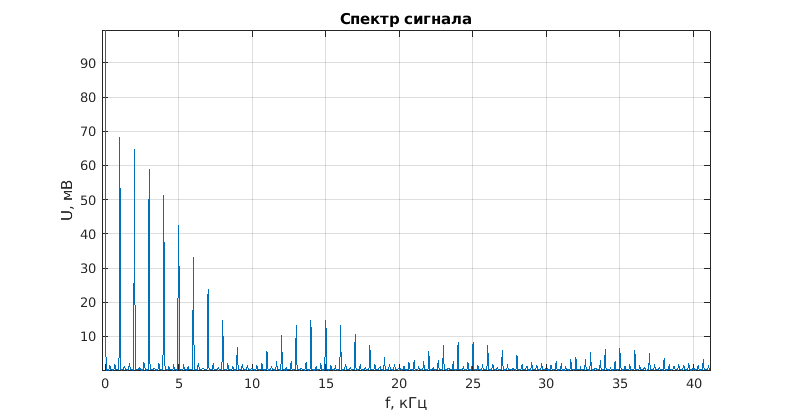
\includegraphics[width = 14 cm]{images/1_100_1.png}
    \caption{Спектр при $f_{\text{повт}} = 1$ кГц, $\tau = 100$ мкс}
\end{figure}

\begin{figure}[h!]
    \centering
    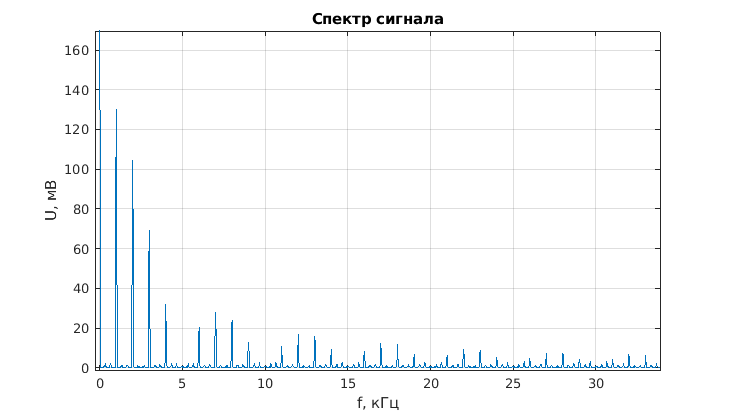
\includegraphics[width = 14 cm]{images/1_200_1.png}
    \caption{Спектр при $f_{\text{повт}} = 1$ кГц, $\tau = 200$ мкс}
\end{figure}

\begin{figure}[h!]
    \centering
    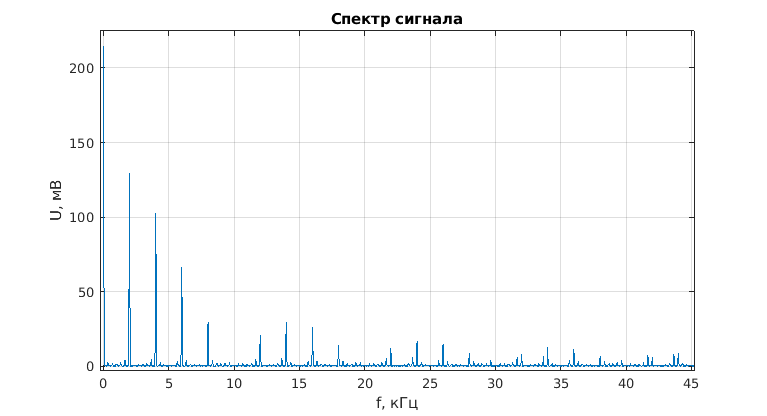
\includegraphics[width = 14 cm]{images/1_100_2.png}
    \caption{Спектр при $f_{\text{повт}} = 2$ кГц, $\tau = 100$ мкс}
\end{figure}

\begin{figure}[h!]
    \centering
    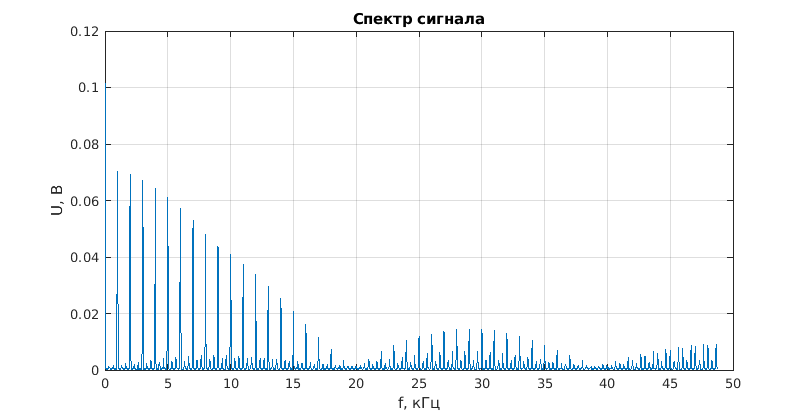
\includegraphics[width = 14 cm]{images/1_50_1.png}
    \caption{Спектр при $f_{\text{повт}} = 1$ кГц, $\tau = 50$ мкс}
\end{figure}

При фиксированной частоте $f_{\text{повт}} = 1$ кГц будем менять $\tau$, при этом будет меняться ширина спектра. Зафиксируем наблюдения в таблице.

\begin{table}[]
    \centering
    \begin{tabular}{|c|l|l|l|l|l|l|l|l|l|}
        \hline
        \textbf{$\tau$, мкс}           & 40 & 60    & 80   & 100 & 120  & 140  & 160  & 180  & 200 \\ \hline
        \textbf{$\Delta \nu$, кГц}     & 25 & 16,5  & 12,5 & 10  & 8,5  & 7    & 6,5  & 5,5  & 5   \\ \hline
        \textbf{$\frac{1}{\tau}$, кГц} & 25 & 16,66 & 12,5 & 10  & 8,33 & 7,14 & 6,25 & 5,56 & 5   \\ \hline
    \end{tabular}
    \caption{Зависимость ширины спектра от времени длительности импульса}
\end{table}

Построим график зависимости $\Delta \nu (\frac{1}{\tau})$:

\begin{figure}[h!]
    \centering
    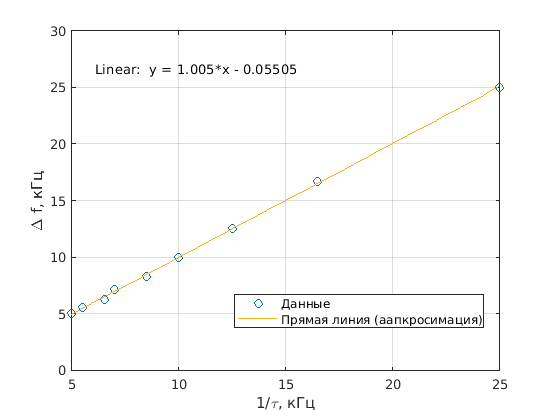
\includegraphics[width = 13 cm]{images/1_appr.png}
    \caption{Зависимость $\Delta \nu (\frac{1}{\tau})$}
\end{figure}

Из графика следует выоплнение соотношения неопределённости для прямяугольных импульсов: $\Delta \nu \cdot \tau = \approx 1$.

\subsection{Периодическая последовательность цугов}

Установим несущую частоту цугов $\nu_0 = 25$ кГц, частота запуска цугов $f_{\text{повт}} = 1$ кГц с длительностью импульса $\tau = 100$ мкс.

Проанализируем, как меняется спектр при изменении длительности импульса цуга.

\begin{figure}[h!]
    \centering
    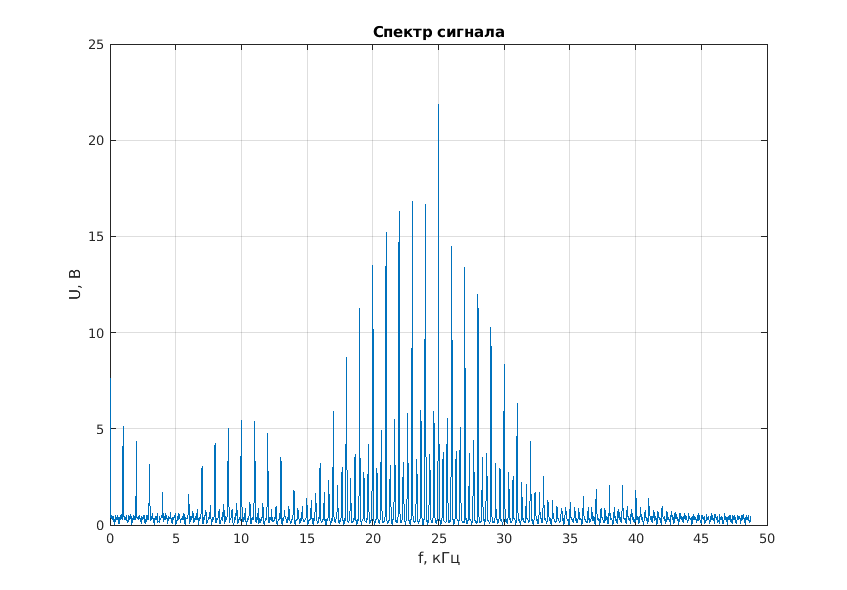
\includegraphics[width = 14 cm]{images/2_100_1.png}
    \caption{Спектр при $\nu_0 = 25$ кГц, $\tau = 100$ мкс}
\end{figure}

\begin{figure}[h!]
    \centering
    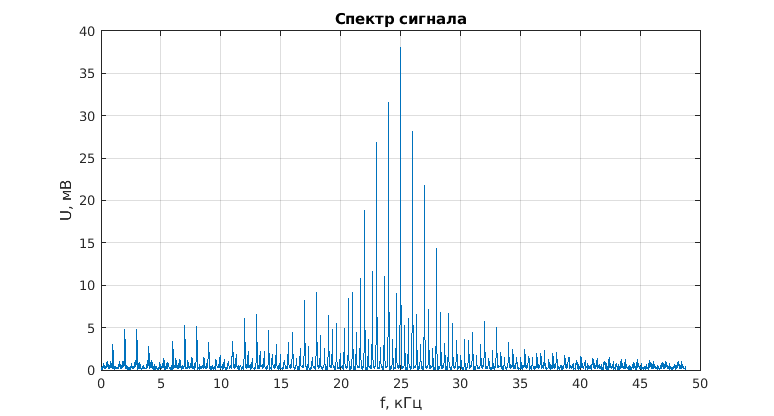
\includegraphics[width = 14 cm]{images/2_200_1.png}
    \caption{Спектр при $\nu_0 = 25$ кГц, $\tau = 200$ мкс}
\end{figure}

Теперь проанализируем, как меняется спектр при изменении несущей частоты.

\begin{figure}[h!]
    \centering
    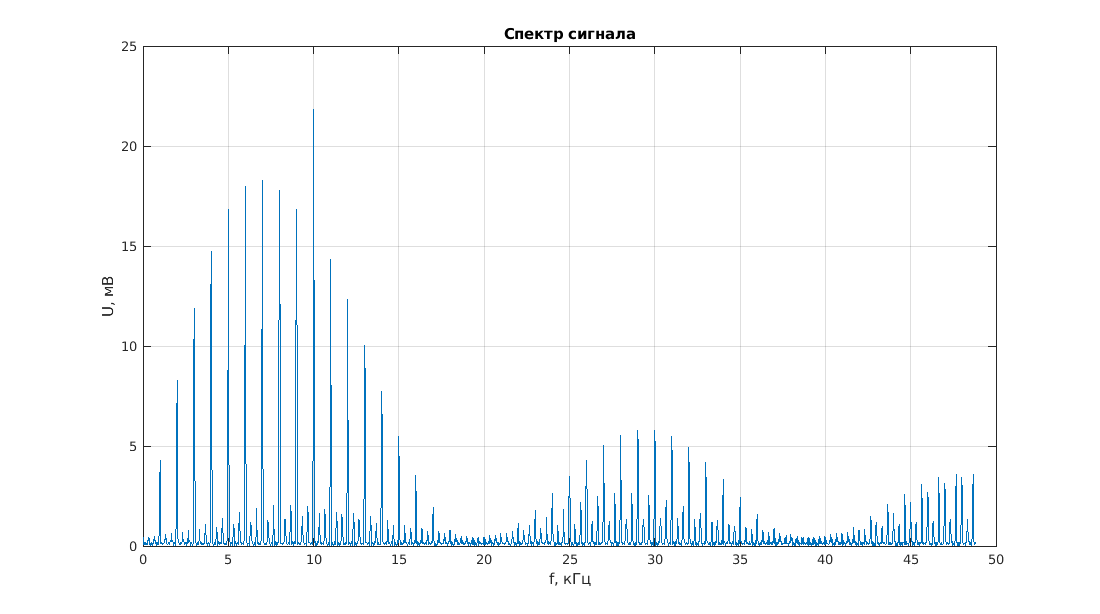
\includegraphics[width = 14 cm]{images/2_10k.png}
    \caption{Спектр при $\nu_0 = 10$ кГц, $\tau = 100$ мкс}
\end{figure}

\begin{figure}[h!]
    \centering
    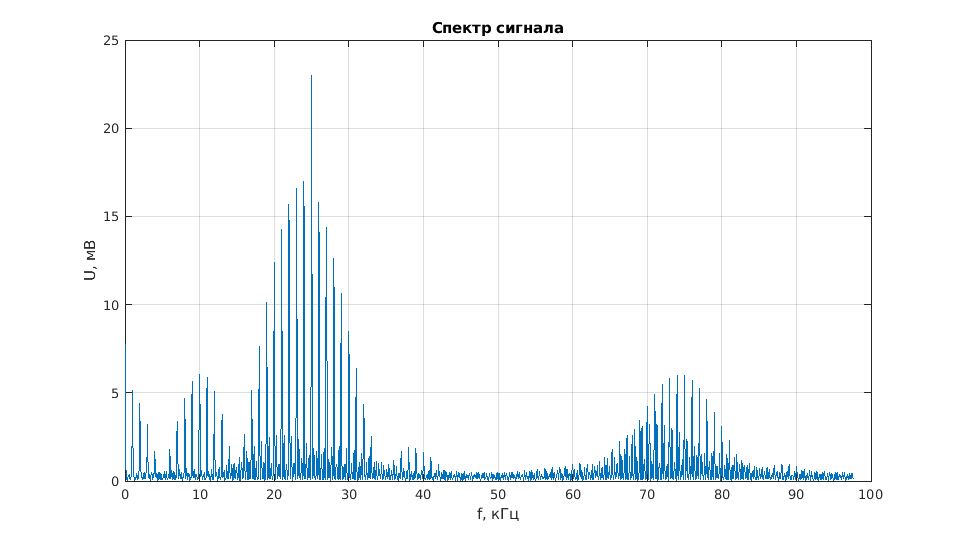
\includegraphics[width = 14 cm]{images/2_25k.png}
    \caption{Спектр при $\nu_0 = 25$ кГц, $\tau = 100$ мкс}
\end{figure}

\begin{figure}[h!]
    \centering
    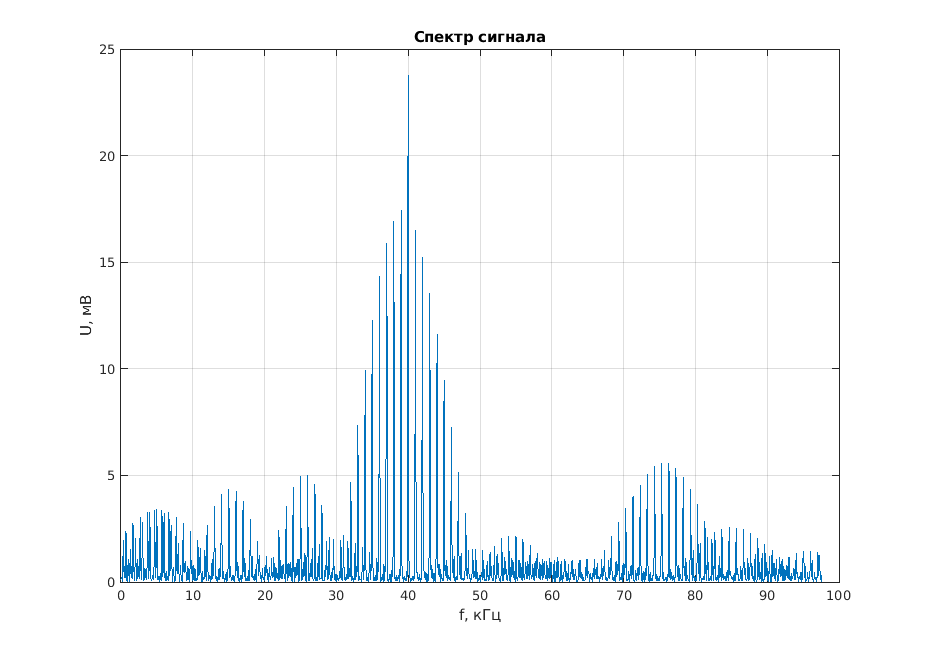
\includegraphics[width = 14 cm]{images/2_40k.png}
    \caption{Спектр при $\nu_0 = 40$ кГц, $\tau = 100$ мкс}
\end{figure}

Установим несущую частоту $\nu_0 = 30$ кГц при $\tau = 100$ Гц, варируя частоту запуска цугов. Снимем зависиимость расстояния между соседними спектральными компонентами от частоты повтоения цугов:

\begin{table}[]
    \centering
    \begin{tabular}{|c|l|l|l|l|l|l|l|l|l|}
        \hline
        \textbf{$\delta \nu$, кГц}      & 0,5 & 1  & 2 & 4  & 5  \\ \hline
        \textbf{$f_{\text{повт}}$, кГц} & 0,5 & 1  & 2 & 4  & 5  \\ \hline
    \end{tabular}
    \caption{Зависимость расстояния между компонентами спектра от частоты повторения цугов}
\end{table}

Данные по расстоянию между компонентами спектра получены по более, чем 80 точек данных, и с точностью до погрешности генератора совпадают со значениями частоты повторения цугов $f_{\text{повт}}$.

Получается, что $\delta \nu = k f_{\text{повт}}$, где $k \approx 1$. Из теории следует, что значения двух величин совпадают, значит экспериментальная зависимость верна.

И для прямугольных импульсов, и для цугов при повышении частоты повторения импульсов увеличивается расстояние между компонентами спектра, а при повышении длительности импульса уменьшается ширина спектра. Разница между графиками спектров прямугольного импульса и цуга в том, что спектр цугаа смещён на значение несущей частоты в сторону поовышения частоты. То есть при устрмлении несущей частоты к нулю графики наложатся друг на друга.

\subsection{Амплитудно-модулированные колебания}

Установим синусоидальный сигнал частоты $\nu_0 = 25$ кГц, амплитуды $0,5$ В. Подключим модуляцию к этому сигналу амплитуды $0,1$ В и частоты $\nu = 1$ кГц.

Меняя глубину модуляции до 1, измерим следующие значения:

\begin{table}[h!]
    \centering
    \begin{tabular}{|c|c|c|c|c|c|c|c|}
        \hline
        \textbf{$A_{min}$, мВ}                           & 450   & 375   & 300   & 225   & 150   & 75    & 0     \\ \hline
        \textbf{$A_{max}$, мВ}                           & 550   & 625   & 700   & 775   & 850   & 925   & 1000  \\ \hline
        \textbf{$m$}                                     & 0,1   & 0,25  & 0,4   & 0,55  & 0,7   & 0,85  & 1     \\ \hline
        \textbf{$A_{\text{бок}}$, мВ}                    & 17    & 43    & 68    & 94    & 120   & 147   & 174   \\ \hline
        \textbf{$A_{\text{осн}}$, мВ}                    & 343   & 341   & 342   & 342   & 340   & 342   & 341   \\ \hline
        \textbf{$\frac{A_{\text{бок}}}{A_{\text{осн}}}$} & 0,496 & 0,126 & 0,199 & 0,275 & 0,353 & 0,430 & 0,510 \\ \hline
    \end{tabular}
    \caption{Зависимость $\frac{A_{\text{бок}}}{A_{\text{осн}}}$ от $m$}
\end{table}

Построим график зависимости.

\begin{figure}[h]
    \centering
    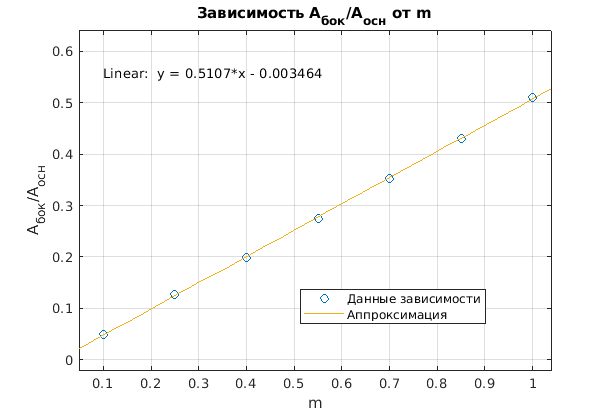
\includegraphics[width = 13 cm]{images/3_appr.png}
    \caption{График зависимости $\frac{A_{\text{бок}}}{A_{\text{осн}}}$ от $m$}
\end{figure}

Получилось значение $k = 0,511 \pm 0,021$, согласно же теории это значение должно равняться $0,5$. То есть получилось верное соотношение амплитуд при различных модуляциях.

При увеличении частоты модуляции две боковые гармоники отдаляются от основной по величине на спектре.

\subsection{Частотная модуляция}

Установим синусоидальный сигнал с частотой $\nu = 25$ кГц с синусоидальной модуляцией частоты $1$ кГц с девиацией частоты $100$ Гц.

Меняя девиацию, снимем зависимость амплитуд гармоник от её значения.

\begin{table}[h!]
    \centering
    \begin{tabular}{|c|c|c|c|c|c|c|c|l|l|l|}
        \hline
        \textbf{$\Delta f_m$, кГц}       & 0,1   & 0,2   & 0,3   & 0,4   & 0,5   & 0,6   & 0,7   & 0,8   & 0,9   & 1     \\ \hline
        \textbf{$A_0$, мВ}               & 338   & 335   & 331   & 325   & 318   & 309   & 299   & 287   & 273   & 260   \\ \hline
        \textbf{$A_{+-1}$, мВ}           & 17    & 33    & 50    & 67    & 83    & 97    & 112   & 125   & 138   & 150   \\ \hline
        \textbf{$A_{+-2}$, мВ}           & 0     & 2     & 4     & 7     & 10    & 15    & 20    & 26    & 32    & 38    \\ \hline
        \textbf{$\beta$}                 & 0,1   & 0,2   & 0,3   & 0,4   & 0,5   & 0,6   & 0,7   & 0,8   & 0,9   & 1     \\ \hline
        \textbf{$\frac{A_{+-1}}{A_{0}}$} & 0,050 & 0,099 & 0,151 & 0,206 & 0,261 & 0,314 & 0,375 & 0,436 & 0,505 & 0,577 \\ \hline
    \end{tabular}
\end{table}

Построим график зависимости $\frac{A_{+-1}}{A_{0}}$ от $\beta$:

\begin{figure}[h!]
    \centering
    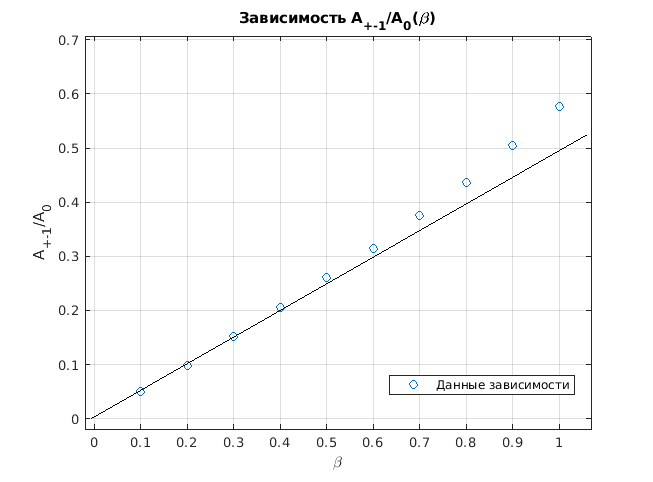
\includegraphics[width = 13 cm]{images/4_appr.png}
    \caption{График зависимости $\frac{A_{+-1}}{A_{0}}$ от $\beta$}
\end{figure}

Предельная кривая, построенная при $\beta \ll 1$, даёт отношение боковых гармоник к основной $k = 0,5$, что и соответсвуте теоретической формуле, выведенной в приближении $\beta \ll 1$. При этом значения $\beta \geqslant 0,9$ дают отклонение от построенной прямой больше, чем $10$ \%.

При дальнейшей увеличении частоты девиации получим более сложные спектры:

\begin{figure}[h!]
    \centering
    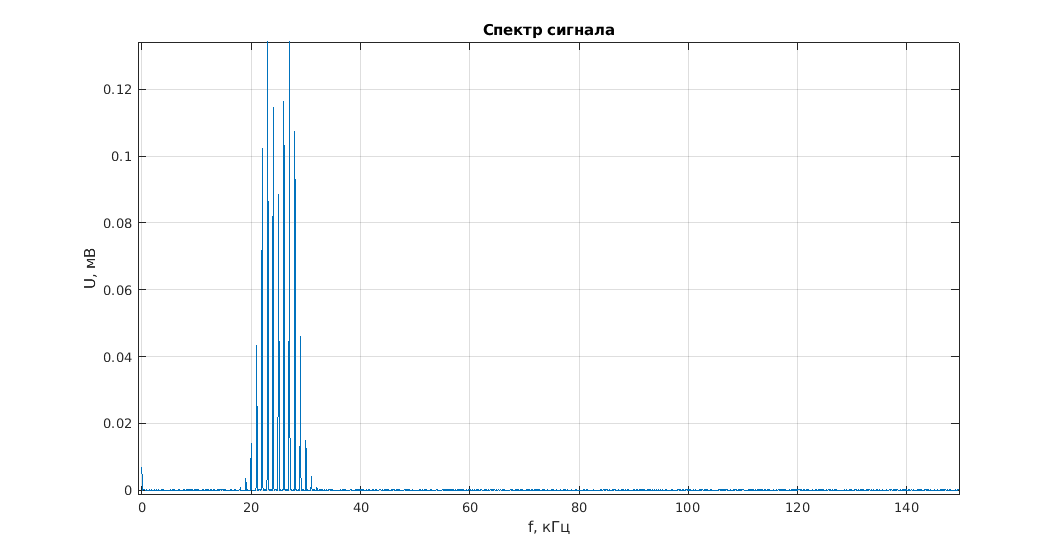
\includegraphics[width = 15 cm]{images/4_3.png}
    \caption{Спектр при частоте девиации $\Delta f_m = 3$ кГц}
\end{figure}

\begin{figure}[h!]
    \centering
    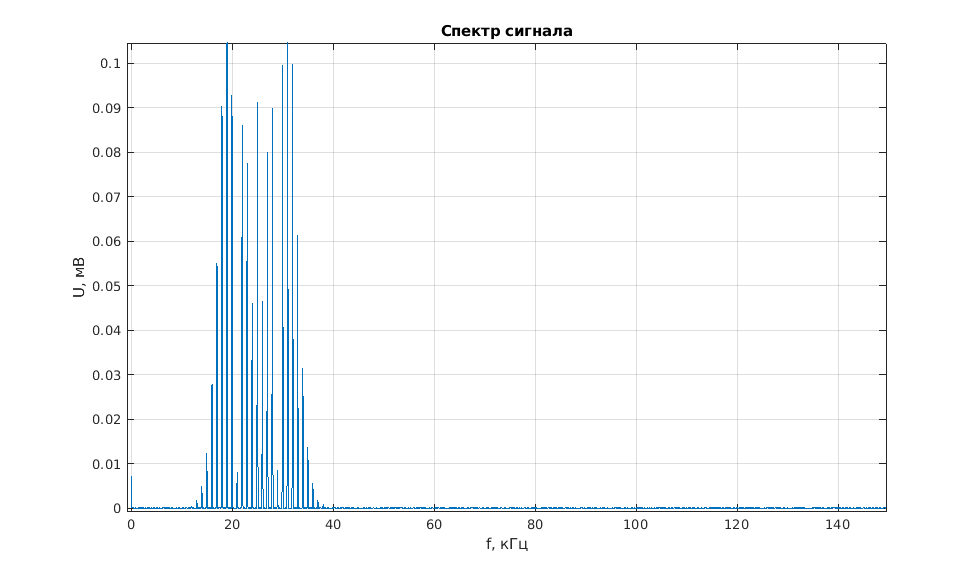
\includegraphics[width = 15 cm]{images/4_7.5.png}
    \caption{Спектр при частоте девиации $\Delta f_m = 7,5$ кГц}
\end{figure}

\section{Заключение}

Таким образом теоретическое описание спектров исследуемых сигналов подтвердилось на основе их изучения с помощью генератора и осциллографа. 











